{\small
\begin{figure}
\centering
\begin{subfigure}{1.0\textwidth}
\begin{centering}
$
    \begin{array}{l}
    \kw{towRounds(k)} \triangleq \\
           \clabel{ \assign{a}{0}}^{0} ;
            \clabel{\assign{j}{k} }^{1} ;\\
            \ewhile ~ \clabel{j > 0}^{2} ~ \edo ~ 
            \Big(
             \clabel{\assign{x}{\query(\chi[j] \cdot \chi[k])} }^{3}  ; 
             \clabel{\assign{j}{j-1}}^{4} ;
            \clabel{\assign{a}{x + a}}^{5}       \Big);\\
            \clabel{\assign{l}{\query(\chi[k]*a)} }^{6}
        \end{array}
$
\caption{}
\end{centering}
\end{subfigure}
\begin{subfigure}{.5\textwidth}
%}
\qquad
\begin{centering}
\begin{tikzpicture}[scale=\textwidth/15cm,samples=200]
\draw[] (0, 10) circle (0pt) node
{{ $a^0: {}^{\lambda \trace_0. 1}_{0}$}};
\draw[] (0, 7) circle (0pt) node
{\textbf{$x^3: {}^{\lambda \trace_0. \env(\trace_0) k}_{1}$}};
\draw[] (0, 4) circle (0pt) node {{ $a^5: {}^{\lambda \trace_0. \env(\trace_0) k}_{0}$}};
\draw[] (0, 1) circle (0pt) node
{{ $l^6: {}^{\lambda \trace_0. 1}_{1}$}};
% Counter Variables
\draw[] (8, 9) circle (0pt) node {\textbf{$j^1: {}^{\lambda \trace_0. 1}_{0}$}};
\draw[] (8, 6) circle (0pt) node {{ $j^4: {}^{\lambda \trace_0. \env(\trace_0) k}_{0}$}};
%
% Value Dependency Edges:
\draw[ ultra thick, -latex, densely dotted,] (0, 1.5)  -- (0, 3.5) ;
\draw[ ultra thick, -latex, densely dotted,] (0, 4.5)  -- (0, 6.5) ;
\draw[ -latex] (0, 4.5)  to  [out=-230,in=230]  (0, 9.5) ;
\draw[ -Straight Barb] (1.5, 3.8) arc (120:-200:1);
\draw[ -Straight Barb] (9, 6.5) arc (150:-150:1);
\draw[ -latex] (8, 6.5)  -- (8, 8.5) ;
\draw[ -latex] (0, 1.5)  to  [out=-230,in=230]  (0, 9.5) ;
% Control Dependency
\draw[ -latex] (2, 7)  -- (6, 9) ;
\draw[ -latex] (2, 7)  -- (5.5, 6) ;
\draw[ -latex] (2, 4.5)  -- (6, 9) ;
\draw[ -latex] (2, 4.5)  -- (5.5, 6) ;
% Edges Produced By Transitivity
\draw[ -latex] (2, 1)  -- (6, 9) ;
\draw[ -latex] (2, 1)  -- (5.5, 6) ;
\draw[ -latex] (0, 1.5)  to  [out=50,in=-50]  (0, 6.5) ;
\end{tikzpicture}
\caption{}
\end{centering}
\end{subfigure}
   \begin{subfigure}{.45\textwidth}
   \begin{centering}
   \begin{tikzpicture}[scale=\textwidth/15cm,samples=200]
\draw[] (0, 10) circle (0pt) node
{{ $a^0: {}^1_{0}$}};
\draw[] (0, 7) circle (0pt) node
{\textbf{$x^3: {}^{k}_{1}$}};
\draw[] (0, 4) circle (0pt) node
{{ $a^5: {}^{k}_{0}$}};
\draw[] (0, 1) circle (0pt) node
{{ $l^6: {}^{1}_{1}$}};
% Counter Variables
\draw[] (6, 9) circle (0pt) node {\textbf{$j^1: {}^{1}_{0}$}};
\draw[] (6, 6) circle (0pt) node {{ $j^4: {}^{k}_{0}$}};
%
% Value Dependency Edges:
\draw[ ultra thick, -latex, densely dotted,] (0, 1.5)  -- (0, 3.5) ;
\draw[ ultra thick, -latex, densely dotted,] (0, 4.5)  -- 
(0, 6.5) ;
\draw[  -latex] (0, 4.5)  to  [out=-230,in=230]  
(0, 9.5) ;
\draw[  -Straight Barb] (1.5, 3.5) arc (120:-200:1);
\draw[  -Straight Barb] (6.5, 6.5) arc (150:-150:1);
\draw[  -latex] (6, 6.5)  -- (6, 8.5) ;
% Control Dependency
\draw[ -latex] (1.5, 7)  -- (5, 9) ;
\draw[ -latex] (1.5, 4)  -- (5, 9) ;
\draw[ -latex] (1.5, 7)  -- (5, 6) ;
\draw[ -latex] (1.5, 4)  -- (5, 6) ;
\draw[  -latex] (0, 1.5)  to  [out=-230,in=230]  (0, 9.5) ;
% Edges Produced By Transitivity
\draw[ -latex] (2, 1)  -- (5, 9) ;
\draw[ -latex] (2, 1)  -- (5, 6) ;
\draw[ -latex] (0, 1.5)  to  [out=50,in=-50]  (0, 6.5) ;
\end{tikzpicture}
\caption{}
   \end{centering}
   \end{subfigure}
\vspace{-0.4cm}
 \caption{(a) The program $\kw{towRounds(k)}$, an example 
%  of a program 
with two rounds of adaptivity (b) The corresponding semantics-based dependency graph (c) The estimated dependency graph from $\THESYSTEM$.
}
\label{fig:overview-example}
% \vspace{-0.8cm}
\end{figure}
}
We illustrate the key technical components of our framework through a simple adaptive data analysis with two rounds of adaptivity.
In this analysis, an analyst asks $k+1$ queries to a mechanism in two phases.
In the first phase, the analyst asks $k$ queries and stores the answers that are provided by the mechanism. In the second phase, the analyst constructs a new query based on the results of the previous $k$ queries and sends this query to the mechanism. 
The mechanism is abstract here and our goal is to use static analysis to provide an upper bound on adaptivity to help choose the mechanism.
This data analysis assumes that the data domain $\univ$ 
contains at least $k$ numeric attributes 
(every query in the first phase focuses on one), which we index just by natural numbers.
The implementation of this data analysis in the language of {\THESYSTEM} is presented in Fig.~\ref{fig:overview-example}(a).

\subsection{Program Model}
The {\THESYSTEM} language extends a standard while language\footnote{Programs components are labeled, so that we can uniquely identify every component.} with a query request constructor denoted $\query$. Queries have the form $\query(\qexpr)$, where $\qexpr$ is a special expression 
(see syntax in Section~\ref{sec:language}) representing a function $\from \univ \to U$ on rows.
We use $U$ to denote the codomain of queries and it could be $[-1,1]$, $[0,1]$ or $[-R,+R]$, for some $R$ we consider. This function characterizes the linear query we are interested in running. Indeed, as we discussed in the previous section, linear queries compute the empirical mean of a function on rows --- we use $\chi$ to abstract a possible row in the database.
 As an example, $x \leftarrow \query(\chi[j] \cdot \chi[k])$ computes an approximation, according to the used mechanism, of the empirical mean of the product of the $j^{th}$ attribute and $k^{th}$ attribute, identified by $\chi[j] \cdot \chi[k]$. Notice that we don't materialize the mechanism but we assume that it is implicitly run when we execute the query. 
 In Fig.~\ref{fig:overview-example}(a), the queries inside the while loop correspond to the first phase of the data analysis and compute an approximation of 
the product of the empirical mean of the first $k$ attributes. 
The query outside the loop corresponds to the second phase and computes an approximation of the empirical mean where each record is weighted by the sum of the empirical mean of the first $k$ attributes.


This example is intuitively 2-rounds adaptive since we have two clearly distinguished phases, and the queries that we ask in the first phase do not depend on each other (the query $\chi[j] \cdot \chi[k]$ at line $3$ only relies on the counter $j$ and input $k$), while the last query 
(at line 6) depends on the results of all the previous queries. 
However, capturing this concept formally is surprisingly difficult. The difficulty comes from the fact that a query can depend on the result of another query in multiple ways, by means of data dependency or control flow dependency.
% \mg{this is weaker than it was in the previous submission.}

%%%%%%%%%%%%%%%%%%%%%%%%%%%%%%%%%%%Some details that might be useful when make passes %%%%%%%%%%%%%%%%%
% \jl{ The $\bullet$ stands for no query, for instance, the second event in the trace $(j, 1, \env(\trace)k , \bullet) $ tells us the assignment at line $1$ does not request a query.} \jl{The third event is a testing event corresponding to the guard of the while loop at line $2$. The evaluation of the query request in the second phase is tracked in }
% % \jl{ 
% The $\bullet$ is a default value for non-query event, 
% for instance, the second event in the trace $(j, 1, K , \bullet) $ tells us the assignment at line $1$ does not request a query.
% The third event is a testing event corresponding to the guard of the while loop at line $2$. The evaluation of the query request in the second phase is tracked in 
% % }
\subsection{Adaptivity definition}
\label{sec:adaptivity-informal}
%%%%%%%%%%%%%%%%%%%%%%%%%%%%%%%%%%% Details Below that might be useful when make passes %%%%%%%%%%%%%%%%%
% \detailed{To formally define the adaptivity, we build a directed graph representing the possible dependencies between queries of a program and we call this graph: execution-based dependency graph. The vertices represent the assigned program variables and the edges satisfy the dependency relations between vertices.   Fig.~\ref{fig:overview-example}(b) is the execution dependency graph we build based on the "two rounds strategy program" in Fig.~\ref{fig:overview-example}(a). In brief, the graph is built by collecting the assigned variables with labels of the target program as vertices, which are $a^0$, $j^1$,...$a^5$,$l^6$. We check if there is an edge between two vertices by our dependency relation over two labeled variables (defined in Section~\ref{sec:dep_adaptivity} ). This dependency relation relies on the execution of the program recorded by a trace generated by our trace semantics, which is the reason we call this graph "execution-based". 
% Intuitively from Fig.~\ref{fig:overview-example}(a), the query in the second phase (at line 6) depends on the query results in the first phase stored in $a$ at line 5, and the variable $a$ also relies on the queries at line 3. Correspondingly, we have two edges $(l^6, a^5)$ and $(a^5, x^3)$ in our execution-based dependency graph in Fig.~\ref{fig:overview-example}(b). Besides, we also have special edge which is a circle, to track any variable being updated with its previous value recursively. For instance, the counter $j$ and the variable $a$ are updated based on previous values $k$ times in the first phase and we see two circle edges on $a^5$ and $j^4$.}

The central property we are after in this work is the \emph{adaptivity of a program}. We define formally this notion in three steps, which we will describe in details in Section~\ref{sec:adapt-exe}. First, we define a notion of dependency, or better \emph{may-dependency}, between variables. To do this we take inspiration from previous works on dependency analysis and information flow control and we say that a variable \emph{may depend} on another one if changing the execution of the latter can affect the execution of the former. 
We can see in Fig.~\ref{fig:overview-example}(a) that the value of the variable $l$, which corresponds to the result of the execution of the query in the second phase (in the command with label 6), is affected by the value of the variable $x$, which corresponds to the result of the execution of the query at line 3 in the first phase, via the variable $a$.
To formally define this notion of dependency, as in information flow control, we use the execution history of programs recorded by a trace semantics (see Definition~\ref{def:var_dep}).
% \mg{Please, double check that I refer to the right definition. }  

Second, we build an annotated weighted directed graph representing the possible dependencies between labeled variables. We call this graph \emph{semantics-based dependency graph} to stress that this graph summarize the dependencies we could see if we knew the overall behavior of the program. 
The vertices of the graph are the assigned program variables with the label of their assignments, edges are pairs of labeled variables which satisfy the dependency relations, weights are functions associated with vertexes and describing the number of times the assignment corresponding to the vertex is executed when the program is run in a given starting state\footnote{In our trace semantics the state is recorded in the trace, so an initial state is actually represented by an initial trace. We will use this terminology in later sections.}, and the annotations, which we call \emph{query annotations}, are bits associated with vertexes and describing if the corresponding assignment comes from a query (1) or not (0).
The \emph{semantics-based dependency graph} of the $\kw{twoRounds(k)}$ program
we gave in Fig.~\ref{fig:overview-example}(a) is described in Fig.~\ref{fig:overview-example}(b) (we use dashed arrows for two edges that will be highlighted in the next step, for the moment these can be considered similar to the other edges---i.e. solid arrows). We have all the variables that are assigned in the program with their labels, and edges representing dependency relations between them. 
For example, we have two edges $(l^6, a^5)$ and $(a^5, x^3)$ describing the dependency between the variables assigned by queries. The vertices $l^6$ and $x^3$ are the only ones with query annotation $1$ (the subscript), since they are the only two variables that are in assignments involving  queries. Notice that the graph contains cycles---in this example it contains two self-loops. These cycles capture the fact that the variables $a^5$ and $j^4$ are updated at every iteration of the loop using their previous value. Cycles are essential to capture mutual dependencies like the ones that are generated in loops. Adaptivity is a quantitative notion, so capturing this form of dependencies is not enough. This is why we also use weights. The weight of a vertex is a function that given an initial state returns a natural number representing 
the number of times the assignment corresponding to a vertex is visited during the program execution starting in this initial state.  
For example, the vertex $l^{6}$ has weight {$\lambda \trace.1$} since for every initial state {$\trace$} the corresponding assignment will be executed one time, the vertex $a^5$ on the other hand has weight {$\lambda \trace. \env(\trace) k$ since the corresponding assignment will be executed a number of times that correspond to the value of $k$ in the initial state $\trace$, and $\env$ is the operator reading value of $k$ from $\trace$.
}

Third, we can finally define adaptivity using the semantics-based dependency graph. We actually define this notion with respect to an initial state $\tau$, since different states can give very different adaptivity.  We consider the longest walk  that visits each vertex $v$ of the semantics-based dependency graph no more than the value that the weight $w_v$ assign to $\tau$, and visits as many query nodes as possible. The number of query nodes visited is the adaptivity of the program with respect to $\tau$.
Looking again at Fig.~\ref{fig:overview-example}(b), and assuming that $\tau(k) \geq 1$, we can see that the 
the walk along the dashed arrows,  $l^{6} \to a^5 \to x^3 $ has two vertices with query annotation $1$, and we cannot find another walk having more than $2$ vertices with query annotation $1$. So the adaptivity of the program in Fig.~\ref{fig:overview-example}(a) with respect to $\tau$ is $2$. If we consider an initial state $\tau$ such that $\tau(k)=0$ we have that the adaptivity with respect to $\tau$ is instead $1$. 

\subsection{Static analysis}
 %%%%%%%%%%%%%%%%%%%%%%%%%%%%%%% Previous Version Above for Reference  %%%%%%%%%%%%%%%%%
To compute statically a sound and accurate upper bound on the \emph{adaptivity} of a program $c$,
we design a program analysis framework named {\THESYSTEM} which we will describe formally in \ref{sec:adapt-static}. 
The structure of {\THESYSTEM} (Fig.~\ref{fig:adaptfun-overview}) reflects in part the definition of adaptivity we discussed in the previous section. Specifically, {\THESYSTEM} is composed by two algorithms (the ones in dashed boxes in the figure), one for building a dependency graph, which we call \emph{estimated dependency graph}, and the other to estimate the adaptivity from this graph.  
The first algorithm, which we will describe formally in Section~\ref{sec:adapt-static}, generates the \emph{estimated dependency graph} using several program analysis techniques. Specifically, {\THESYSTEM} extracts the vertices and the query annotations by looking at the assigned variables of the program, it estimates the edges by using control flow and data flow analysis, and it estimates the weights by using symbolic reachability-bound analysis---weights in this graph are symbolic expressions over input variables. 
% This combined analysis allow us to obtain more accurate upper bounds than what we would obtain by using any of these single analysis technique in isolation.
The second algorithm estimates the longest walk which respect the weights and which visit as many query nodes as possible. 
The two algorithm together gives us an  upper bound on the program's \emph{adaptivity}.

 \begin{figure}
  \centering    
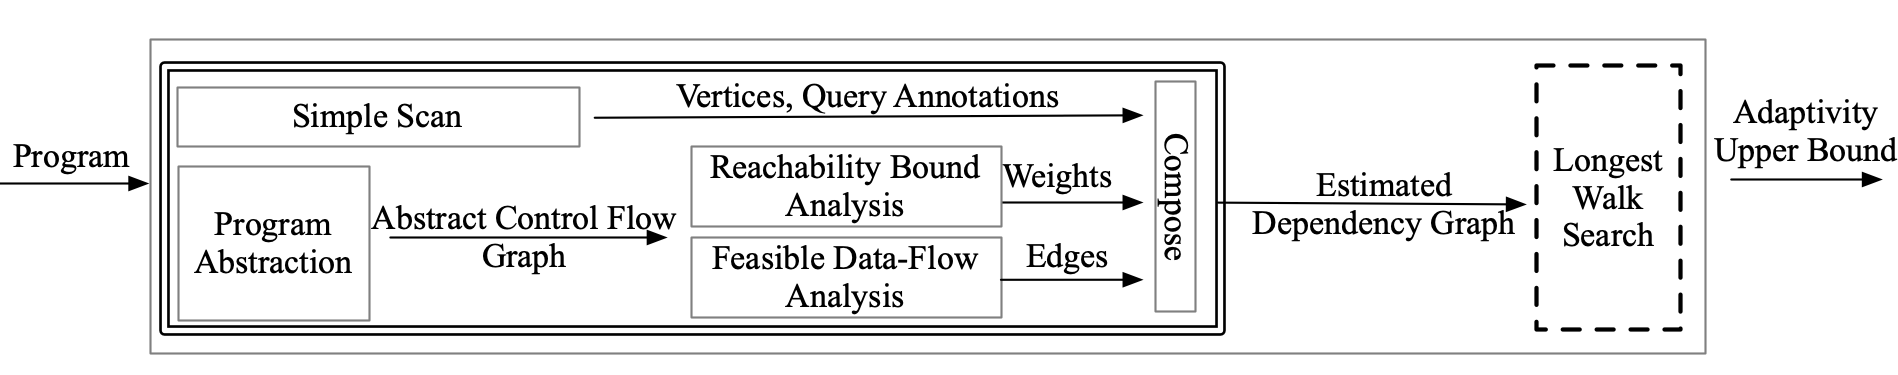
\includegraphics[width=1.0\columnwidth]{adaptfun.png}
  \vspace{-0.8cm}
  \caption{The overview of {\THESYSTEM}}
  \label{fig:adaptfun-overview}
  \vspace{-0.5cm}
\end{figure}

 
%%%%%%%%%%%%%%%%%%%%%%%%%%%%%%%%%%% Details Below that might be useful when others are making passes %%%%%%%%%%%%%%%%%
%   \detailed{Fig.~\ref{fig:overview-example}(c) is the resulting estimated graph of our static analysis algorithm which consumes the program in Fig.~\ref{fig:overview-example}(a).The edges are generated by our graph generation algorithm which combines control flow analysis and data flow analysis, presented in Section~\ref{sec:alg_edgegen}). We can easily see the generated graph in Fig.~\ref{fig:overview-example}(c) is a safe approximation of its execution-based counterpart in Fig.~\ref{fig:overview-example}(b), in the way that we can find a corresponding edge in Fig.~\ref{fig:overview-example}(c) for all the edges in Fig.~\ref{fig:overview-example}(b). We call the weight of every vertex computed by our algorithm as estimated weight,  }
%   estimated by using a reachability-bound estimation algorithm (presented in Section~\ref{sec:alg_weightgen}). \detailed{Different from the execution-based weight $w_1$ or $w_k$ in Fig.~\ref{fig:overview-example}(b) which is a function whose output relies on the initial trace, our estimated weight} can be symbolic and provide a sound upper bound on its execution-based weight of the corresponding vertex in the execution-based dependency graph. For instance, 
%   the estimated weight $k$ of the vertex $x^{3}$ in Fig.~\ref{fig:overview-example}(c) is a sound upper bound on the execution-based weight $w_k$ of vertex $x^{3}$ in Fig.~\ref{fig:overview-example}(b), with the same starting trace $\trace$, $w_k(\trace) \leq\trace(k)$. $\trace(k)$ means getting the value of variable $k$ in the trace $\trace$. The soundness of this step is proved in Theorem~\ref{thm:addweight_soundness}.   
%
We show in Fig.~\ref{fig:overview-example}(c) the estimated dependency graph that our static analysis algorithm returns for the program $\kw{twoRounds(k)}$ in Fig.~\ref{fig:overview-example}(a).
Vertices and query annotations are the same as the ones in Fig.~\ref{fig:overview-example}(b) and they are simply inferred by scanning the program.
As we said before, the edges are estimated using control flow and data flow analysis.
For the $\kw{twoRounds(k)}$ example, every edge in Fig.~\ref{fig:overview-example}(b) is precisely inferred by our combined analysis, this is why Fig.~\ref{fig:overview-example}(c) contains exactly the same edges.
The weight of every vertex is computed using a reachability-bound estimation algorithm which output a symbolic expression over the input variables, in the example only $k$, representing an upper bound on the number of times each assignment is executed.
% \wq{symbolic and provide a sound upper bound on its execution-based weight of the corresponding vertex in the execution-based dependency graph.
% $w_k(\trace) \leq \trace(k)$. $\trace(k)$ means getting the value of variable $k$ in the trace $\trace$. The soundness of this step is proved in Theorem~\ref{thm:addweight_soundness}.}
For example, consider the vertex $x^{3}$, its weight is $k$ and this provides an upper bound on the values returned by the weight function $\lambda \trace. \rho(\trace)k$ associated with vertex $x^{3}$ in Fig.~\ref{fig:overview-example}(b) for any initial state. 
% Indeed, 
% for any initial trace $\trace_0$, when $w_{x^{3}}(\trace_0)$ executes the program and counts the
% execution times of command $3$,
% we expect that this counts is at most the the loop iterations, i.e. $k$'s initial value from $\trace_0$.

The algorithm searching for the longest walk first finds a path $l^6:{}^1_1 \to a^5: {}^k_1 \to x^3: {}^k_1$, and then constructs a walk based on this path. Every vertex on this walk is visited once, and the number of vertices with query annotation $1$ in this walk is $2$, which is the upper bound we expect.
{It is worth to note here that $x^3$ and $a^5$ can only be visited once because there isn't an edge to go back to them, even though they both have the weight $k$}.
In this sense, instead of simply computing the weighted length of this path ($2k+1$) as adaptivity $\pathsearch$ computes the upper bound $2$. Note that $2$ is not always tight, for example when $k = 0$.
